% possible refs
%  - https://www.spiedigitallibrary.org/conference-proceedings-of-spie/10445/104455S/Compensation-of-hard--and-soft-iron-distortions-is-magnetometer/10.1117/12.2280794.short
%  - https://www.mathworks.com/help/nav/ref/magcal.html

% this chapter could be split into
%  - (overview)
%  - problem description
%  - related work

% mention that this thesis is about magnetostatics? since building, earth and phone field is changing very slowly (and em waves are far too weak?)

% compare particle filter approach to existing methods
%  - there are some reference about methods in the madgwick internal report

The hard iron effect in the smartphone is caused by magnetic materials inside the phone which retain their magnetism even after the removal of the external magnetic fields. A permanent magnet of a speaker inside the phone, or inside the vibration unit are examples for that. Since the magnetization of the materials can still change in strength and direction in presents of external fields, this is a dynamical effect and therefore needs continuous calibration.

\begin{figure}[hbt!]
    \centering
    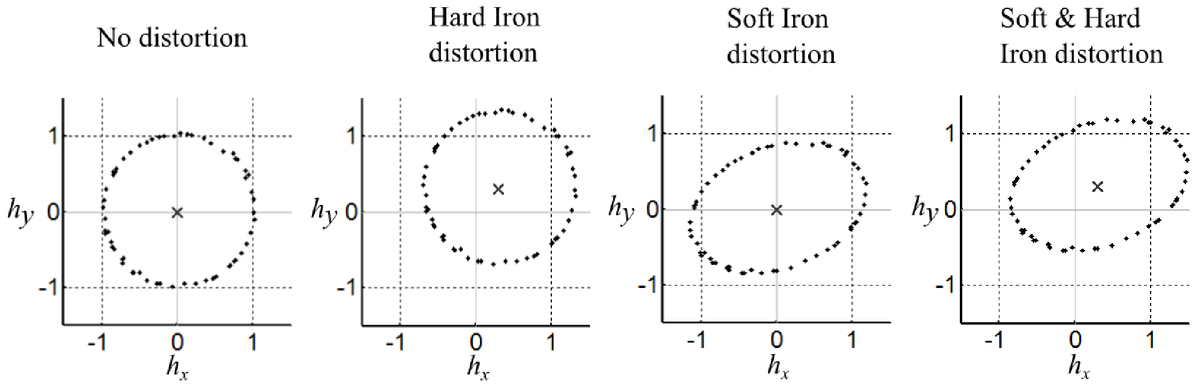
\includegraphics[width=0.6\textwidth]{figures/hard_soft_iron.jpg}
    \caption{Illustration of the hard and soft iron effect.\cite{hard_soft_iron}}
    \label{fig:hard_soft_iron}
\end{figure}

Figure \ref{fig:hard_soft_iron} is an example of how hard and soft iron effects influence the measurement of the magnetometer after a full rotation along an arbitrary axis.

Usually, the hard iron calibration done by the operating system or manufacturer and therefore depending on different algorithms across different devices. Treating the estimates equally is an additional source of error. Apart from that, the operating system does not quantify the quality of the hard iron calibration and requires unnatural movements of the phone to progress the calibration.

The measurement of the magnetic flux density vector by the magnetometer can be expressed by the following.

\begin{equation}
\label{eq:decomposition}
    \bm{B}_{measure} = \bm{B} + \bm{B}_{noise} = \bm{B}_{phone} + \bm{B}_{earth} + \bm{B}_{env} + \bm{B}_{noise}
\end{equation}

Where $\bm{B}_{measure}$ is the measurement of the magnetometer at a given point in time, $\bm{B}_{noise}$ the noise produced by the magnetometer, $\bm{B}_{phone}$ the magnetic field created by the device, $\bm{B}_{earth}$ the magnetic field of the earth, and $\bm{B}_{env}$ is the true ambient magnetic field of the environment.

Let us imagine to rotate the phone in any direction to understand how the individual components change. Assuming that $\bm{B}_{noise}$ is isotropic it will not change. In the frame of reference of the phone, $\bm{B}_{earth}$ and $\bm{B}_{env}$ will be rotated in the opposite direction. The magnetic field of the device $\bm{B}_{phone}$ is created by components of the interior which are firmly connected to the magnetometer. Therefore $\bm{B}_{phone}$ is constant in the frame of reference of the device.

Since $\bm{B}_{earth}$ and $\bm{B}_{env}$ behave in the same way under rotation of the device, we can already guess that the full decomposition is a non trivial problem. Assuming we know the horizontal and vertical component of $\bm{B}_{earth}$ (those could be calculated with the dipole approximation of the Earth's magnetic field) it only depends on the horizontal orientation of the device. Without any model for $\bm{B}_{env}$ the decomposition is ambiguous in all directions. Such a model would make assumptions about the magnitude (for example $\lVert \bm{B}_{env} \rVert << \lVert \bm{B}_{earth} \rVert$) or direction (for example random directions) for the ambient magnetic field of the environment.

Common calibration techniques are:

\begin{itemize}
  \item Static calibration. The device is rotated in all directions while measuring the magnetic field and orientation of the device. A numerical fit can be used to estimate the hard iron effect and these values will later be used in the application to correct the measurements.
  \item Calibration by significant rotation. An algorithm detects when the phone is rotated significantly in multiple directions and uses the same approach as above to estimate the hard iron effect.
\end{itemize}
